\chapter{Development of a device for direct counting of the number of beam particles}

\section{Introduction}
This chapter will focus on the devices under development within the MoVeIT project in order to obtain a single proton counting device.
This comprehends a solid state detector, the Application Specific Integrated Circuits (ASICs) used to digitalise the signal and the final read-out board.
\begin{figure}[H]
	\centering
	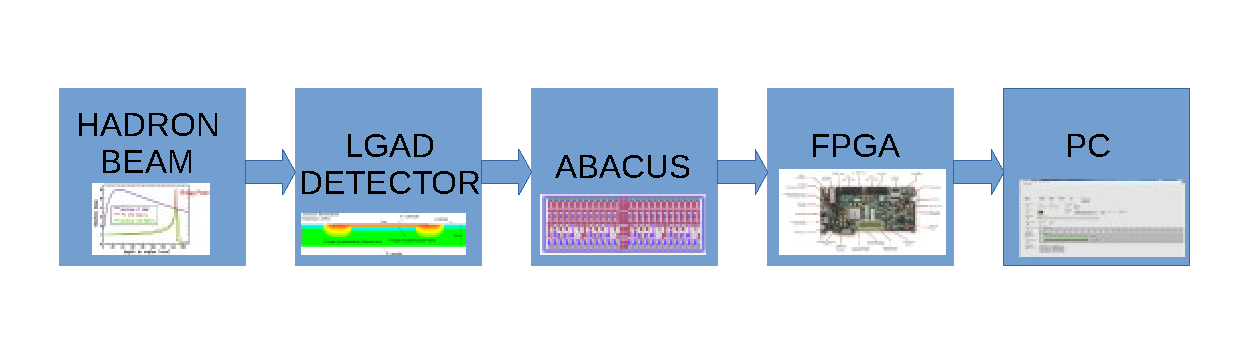
\includegraphics[width=0.99\linewidth]{IMG/ch2/BLOCK}
	\caption{Data flow, from beam to pc.}
	\label{fig:block}
\end{figure}
\noindent In figure \ref{fig:block} it can be seen a diagram with the "data flow" of the project.
The particle beam coming from the accelerators are detected by a Low Gain Avalanche Diode (LGAD) sensor that will be discussed in section \ref{lgad}, the current signal coming from the detector is then amplified and digitalized by the second version of a full custom circuit named ABACUS2 that will be discussed in section \ref{chip}.
This ASIC will be mounted on a full custom PCB referred as Esa-Abacus that will be analysed in section \ref{esaabacus}.
The data from the chip are then read by an Field Programmable Gate Array (FPGA) board, a general purpose device that will be described in detail within chapter 3.
The FPGA elaborates the data and finally sends them to a computer. In the final operational device the computer, on the base of the counted particles, should move and control the beam in a close and controlled loop. 
\newpage
\begin{figure}[H]
	\centering
	
\includegraphics[width=0.35\linewidth]{IMG/ch2/Move_IT_logo}
	%\caption{}
	%\label{fig:moveit}
\end{figure}
\section{The MoVeIT project}\label{moveit}
\noindent The Medical Physics group at University of Turin and INFN (the Italian National Institute for Nuclear and Particle Physics) currently are participating to the Modeling and Verification for Ion beam Treatment planning research project (MoVeIT), which aims to develop new and innovative models for biologically optimized Treatment Planning Systems (TPS) using ion beams in hadron therapy\cite{moveit}.
As~part of the project the Turin group is involved in the development of solid state detectors and readout electronics for measuring with high precision
the characteristics of the hadron beam for irradiation, such as number of particles delivered per unit time, energy and beam profile.
The final goal is to prove the ability of LGAD detectors to discriminate individual protons and to count their number up to fluxes of 100~MHz/cm$^2$ with an uncertainty below 1\% which is the required clinical tolerance.
In order to do that a custom detector was built specifically for this purpose; a LGAD type sensor with an area of $\approx$ 3x3~cm$^2$ and 144 strips which has a thickness of the active region of 50~$\mu$m.
The final goal is to use two of this sensors in orthogonal directions in order to obtain a precise information on the beam position and profile\cite{hammad}.
The main key-points of the final design are:
\begin{itemize}
	\item a cover area of $\approx$ 3x3~cm$^2$;
	\item a maximum measurable flux of 10$^8$~$\frac{p}{s \cdot cm^2}$ with less than 1\% error;
	\item sensitivity of single particle at low fluxes;
	\item provide beam shape in two orthogonal directions.
\end{itemize}


\section{Low Gain Avalanche Diode (LGAD)}\label{lgad}
\noindent The first device involved is the sensor.
short signals are mandatory in order to be able to detect a single particle and to reduce the pile-up effects.
To obtain a short signal the active region of the sensor needs to be the as thin as possible. However the thinner the detector the lower is the Signal to Noise Ratio (SNR).
To solve this problem it was decided to use a new type of sensors known as LGAD.
\noindent Low-Gain Avalanche Detectors (LGADs) are innovative detectors developed in collaboration with the Fondazione Bruno Kessler (FBK, Trento) which feature a moderate ($\approx$10) internal charge multiplication achieved through an additional p+ doping layer few microns depth. The increased signal-to-noise ratio allows designing very thin Ultra Fast Silicon Detectors (UFSD) designed for fast signal collection times, high rates and very good time resolution\cite{lgad}.
%%%%%%%%%%%%%%%%%%%%%%%%%%%%%%%%%%%%%%%%%%%%%%%%%%%%%%%%%%%%%%%%%%%%%%%%%%%%%%%%%%%%%%%%%%%%%%%%%%%%%%%%%%%%%%%%%
The basic doping profiles of the LGAD structure, based on a standard P-In-N detector, is sketched in figure \ref{fig:ufsdlgad}, showing a n++/p+/p/p++ structure.
The figure depicts a highly doped n++ cathode electrode with a moderately doped p+ type region
below, known as the multiplication implant. The n-type electrode has a peak doping concentration
of order 1 $\cdot$ 10$^{19}$ cm$^{-3}$ and has a shallow profile into the bulk of $\approx$ 1 $\mu$m.
The p-type multiplication implant has a peak doping concentration of order 1 $\cdot$ 10$^{16}$ cm$^{-3}$
and has a significantly deeper profile into the bulk ($\approx$ 4 $\mu$m) than the n++ electrode. The bulk
material is high resistivity p-type silicon (approximately 10 k$\Omega$/cm) with a p++ anode electrode
on the backside.
\begin{figure}[H]
	\centering
	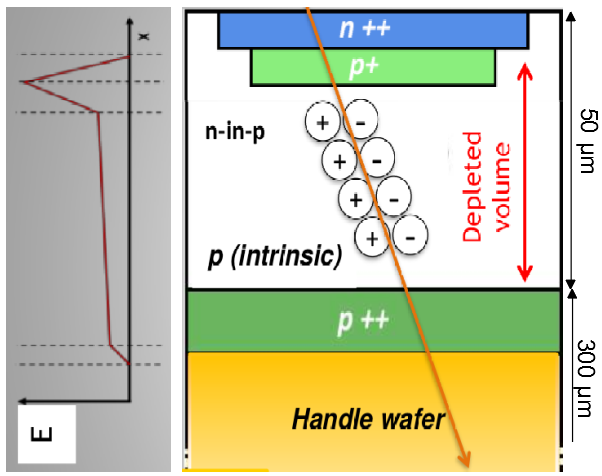
\includegraphics[width=0.35\linewidth]{IMG/ch2/UFSDLGAD.png}
	\caption{Schematic cross-section of the LGAD pad design. A p+ type layer is diffused below the n++ electrode to form the n++/p+/p junction where the multiplication occurs\cite{lgad2}.}
	\label{fig:ufsdlgad}
\end{figure}
\noindent The LGAD device is operated with the bulk fully depleted. Incident radiation produces electron-hole
pairs in the detector which drift towards the cathode and anode respectively. The maximum
electric field in the device is in the junction formed between the n++ cathode and the p+ type multiplication layer and is
proportional to the square root of the p+ type doping density and proportional to the square root of the
external bias voltage for an abrupt junction approximation.
The radiation induced electrons in the detector cross this high field region. For sufficiently
high electric fields impact ionisation occurs which results in multiplication of the carriers therefore a signal gain.
Increasing the high-field (either due to an increase in the doping density or
an increase in the external reverse bias voltage) will increase the electron-hole pair generation rate. For a
low gain device, the goal is to have an overall gain of 10 at $\approx$~200~V bias, with a breakdown voltage
significantly higher than this, at least $\approx$~400~V.
%%%%%%%%%%%%%%%%%%%%%%%%%%%%%%%%%%%%%%%%%%%%%%%%%%%%%%%%%%%%%%%%%%%%%%%%%%%%%%%%%%%%%%%%%%%%%%%%%%%%%%%%%%%%%%%%%
\begin{figure}[H]
	\centering
	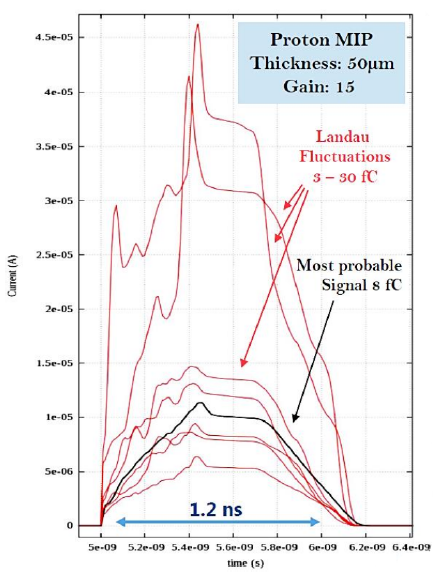
\includegraphics[width=0.42\linewidth]{IMG/ch2/LGAD_Signal}
	\caption{Simulated detector signal\cite{dac}.}
	\label{fig:signal}
\end{figure}
\noindent The output signal from a detector used in the project has a trapezoidal form, a duration of $\approx$ 1.2~ns (rise and fall times of $\approx$~450~ps and a  flat region of $\approx$~300~ps) and a current in the order of 1$\cdot$10$^{-5}$~A.
In figure \ref{fig:signal} it can be seen a signal simulation, the most probable signal carries a 8~fC charge, however due to the Landau fluctuations this value can change between 3~fC and 30~fC.
%%%%%%%%%%%%%%%%%%%%%%%%%%%%%%%%%%%%%%%%%%%%%%%%%%%%%%%%%%%%%%%%%%%%%%%%%%%%%%%%%%%%%%%%%%%%%%%%%%%%%%%%%%%%%%%%%
\noindent The main risk in
the use of LGAD silicon detectors for beam monitoring is related to the high radiation doses from
therapeutic beams. The design of LGAD sensors was optimized for radiation
resistance, and the measurements performed up to now indicate a stable behavior up to 10$^{15}$~n$_{eq}$/cm$^2$ for 50~$\mu$m thick detectors
(this corresponds to a few days of continous irradiation of a therapeutical proton pencil beam).
In general the internal gain of the sensors decreases with the dose, but this can be compensated by raising the bias voltage.
%It is expected that the use of thinner sensors (50~$\mu$m thickness) will decrease the trapping
%probability in the sensors, therefore extending the operative time. Intense work is currently going
%on in the LGAD community to increase the radiation resistance of the sensors. Several
%approaches as alternative dopants and doping profiles are being investigated with the expectation
%to reach a stable behavior up to >1015~n$_{eq}$/cm$^2$ fluencies in the next 1 or 2 years.


\section{ABACUS2 chip}\label{chip}
%\noindent The signal from each detector strip, shown in figure \ref{fig:signal}, is connected to an input channel of the new ABACUS2 full custom chip\cite{abacus}\cite{dac} designed by the Turin INFN group and submitted on October 2020.
\noindent The Charge signals, shown in figure \ref{fig:signal}, amplified in the LGAD sensor are processed by the second version of a full custom Application Specific Integrated Circuit (ASIC) referred as Asynchronous logic Based Analog Counter for Ultra fast Silicon strips (ABACUS2)\cite{abacus}\cite{dac} which was designed by the Turin INFN group and submitted on October 2020.
\begin{figure}[H]
	\centering
	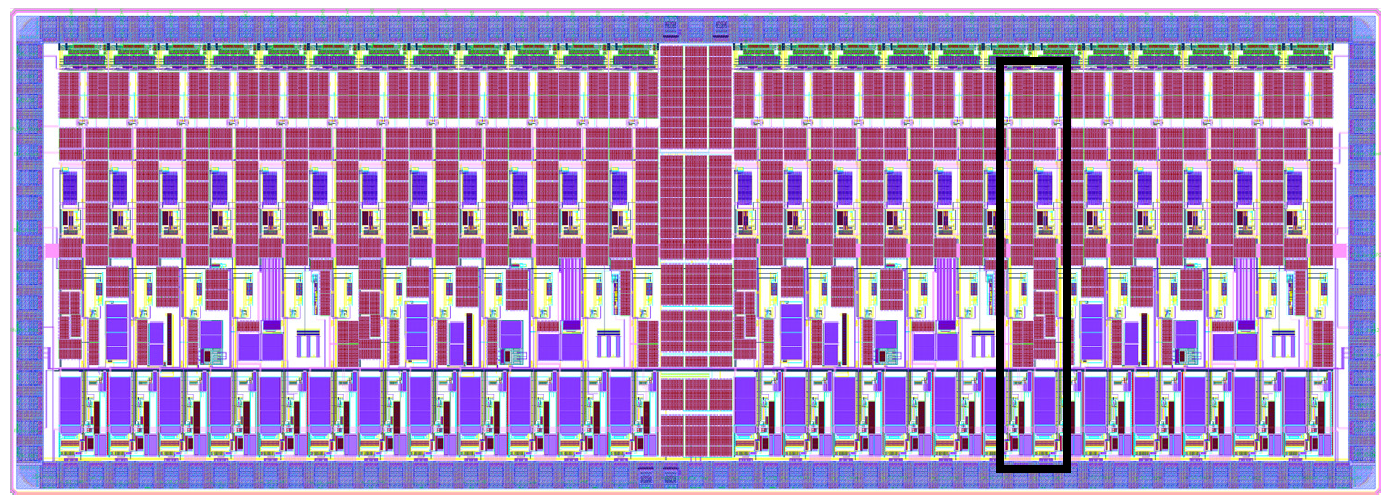
\includegraphics[width=0.9\linewidth]{IMG/ch2/ABACUS2.png}
	\caption{ABACUS2 chip layout.}
	\label{fig:abacus2}
\end{figure}
\noindent In figure \ref{fig:abacus2} it can be seen a schematic of the chip layout.
Inside the black rectangle it can be seen a single channel.
This prototype is a 24 channels ASIC designed in a commercial 110~nm technology.
The die size is 4.95~x~1.935~mm$^2$.
The charge amplification is based on a Regulated Common Gate (RCG) input stage followed by a single stage Trans Impedance Amplifier (TIA).\\
As already discussed, the design goal of the counting device is to measure the number of protons with a maximum uncertainty of 1\% up to a fluxes of 10$^8$~p/(cm$^2$$\cdot$s).
For a single particle the efficiency must be greater than 99\%, and this defines the range of charges the electronics must be able to accept.
The ABACUS2 chip was optimized for an input capacitance between 5 and 20 pF and to cope with continuous signals up to 100 MHz rate.
It can accept input charges from 3~fC to 140~fC, has a dead time <~10~ns and a SNR~>~10.
More details on the channel design are given in the next section. 

\subsection{ABACUS2 Channel structure}
The ABACUS2 chip implements a binary readout system.
A block diagram of a single channel is shown in figure \ref{fig:abacuschannel}.
\begin{figure}[H]
	\centering
	\includegraphics[width=0.8\linewidth]{IMG/ch2/Abacus_channel.png}
	\caption{Single channel diagram of the ABACUS2 chip.}
	\label{fig:abacuschannel}
\end{figure}
\noindent A low noise Charge Sensitive Amplifier (CSA) (1) is followed by a low-pass filter (2).
The output signal from (2) has two components, a DC one, that is called Pedestal, and the actual amplified signal; this will be explained with more details in section \ref{considerations}.
The amplified signal is then fed to a leading-edge multistage discriminator (3 and 4) followed by a driver (5 and 6) which provides a logic pulse in Current Mode Logic (CML) format.
The output of the discriminator is also used in a feedback circuit (7 and 8) to reset the CSA feedback capacitance.
This feedback circuit was designed for a fast baseline restoring and to avoid signal saturation (fast-reset signal).
The chip has been extensively tested by INFN; the output voltage from the amplifier and the noise were estimated by the measurement of the number of detected pulses as a function of the threshold value, this procedure is referred as S-curve method and will be explained is section \ref{considerations}.
The results, in terms of amplifier output voltage as a function of the input charge, are shown in figure \ref{fig:abacustest} for charges between 3 fC and 20 fC\cite{abacus}.
\begin{figure}[H]
	\centering
	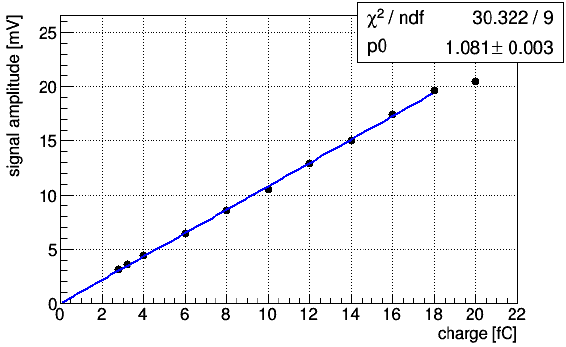
\includegraphics[width=0.7\linewidth]{IMG/ch2/ABACUSTEST}
	\caption{Amplitude of the amplifier output signal as a function of the charge injected at 1 MHz rate.}
	\label{fig:abacustest}
\end{figure}
\noindent For this thesis, the most important considerations concern the functioning of the discriminator (3).
The threshold voltage (V$_{th}$) is the sum of two different components that are independently configurable:
\begin{itemize}
	\item An external 16~bit DAC (Digital to Analog Converter) for the global V$_{th}$;
	\item A programmable 6~bit internal DAC for threshold tuning for each individual channel;
\end{itemize}
\noindent The main external DAC provides the same threshold voltage for every channel, however due to manufacturing tolerances not every channel behaves in the same way.
These differences, which mainly concern the mismatch between the differential pairs of the discriminator, may have a relevant impact on the measured particle rate.
In order to reduce these differences each channel has an independently programmable 6~bit DAC that is used to fine-tune (trim) the V$_{th}$ value.    
\subsubsection{External DAC}
The external DAC is a commercially available Linear Technology LTC2604 Quad 16-bit Rail-to-Rail DAC.
The device uses the Inter Integrated Circuit (I2C) protocol and reads 24~bit words configured as in figure \ref{fig:extdactiming2}.
More details are provided in the data-sheet \cite{LTC2604}.
The main features are:
\begin{itemize}
	\item a guaranteed 16~Bit monotonic characteristic over temperature;
	\item an ultra-low cross-talk between DACs (<~5~$\mu$V);
	\item separate reference inputs for each DAC;
	\item wide 2.5~V to 5.5~V supply range;
	\item low power operation: 250~$\mu$A per DAC at 3~V.
\end{itemize} 
\begin{figure}[H]
	\centering
	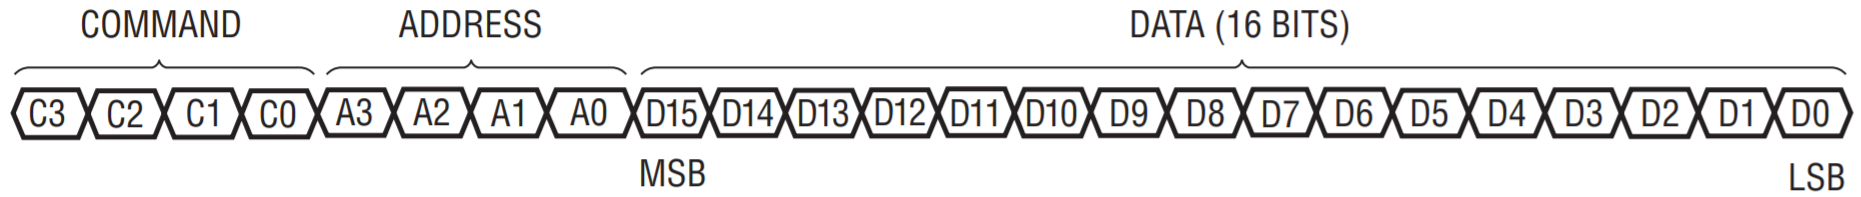
\includegraphics[width=0.99\linewidth]{IMG/ch2/EXTDACTIMING2}
	\caption{24~bit data sequence for the LTC2604 external DAC.}
	\label{fig:extdactiming2}
\end{figure}
\subsubsection{Internal (trimming) DAC}
The internal (trimming) DACs were designed specifically for this chip.
Inside the chip there is an I2C controller used to enable the communication between DAC and the external world.
The DACs are programmed using 16~bit serial words.
The configuration process is explained in detail in section \ref{InternalDac}.
\begin{figure}[H]
	\centering
	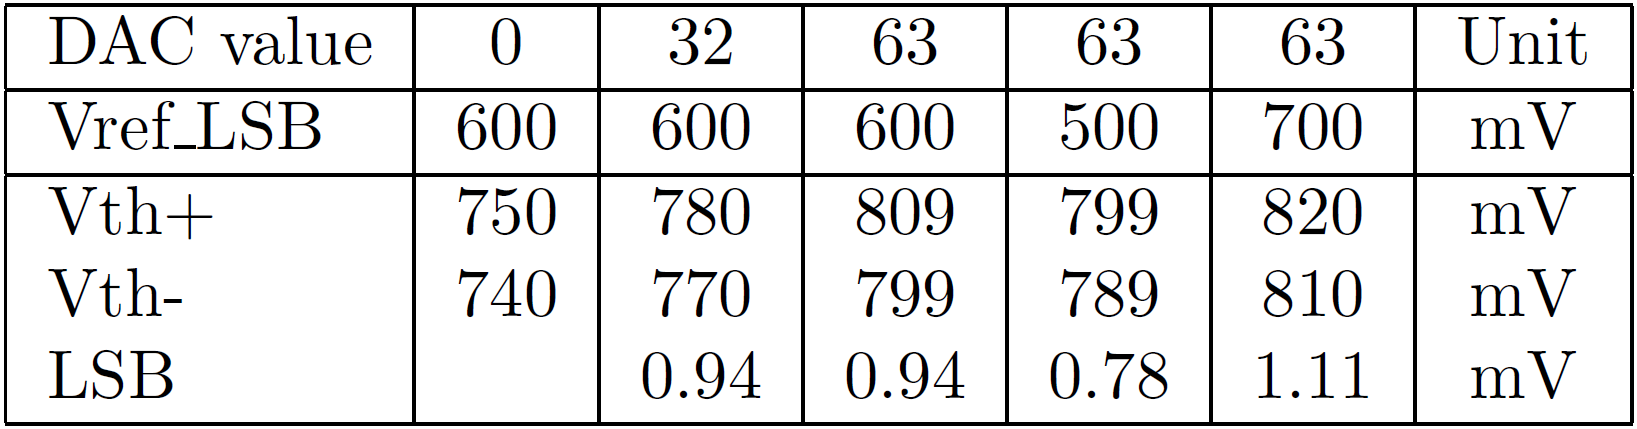
\includegraphics[width=0.5\linewidth]{IMG/ch2/INTDACTABLE}
	\caption{Internal DACs LSB values at different V$_{refLSB}$ settings.}
	\label{fig:intdactable}
\end{figure}
\noindent In figure \ref{fig:intdactable} it can be seen that with a reference voltage of 600~mV the Least Significant Bit (LSB) should be 0.94~mV.
This means that, being this a 6~bit DAC, the maximum trimming voltage is $\approx$~59.2~mV.
For reference, a typical value for the pedestal voltage is $\approx$~560~mV.
Thus these internal DACs are used to fine tune the threshold voltage of the discriminator, while the bulk of the work is done by the external one.   

\section{ABACUS single chip test board}
The ABACUS2 chip was tested using a custom built test board that will be analysed in section \ref{testboard} and a Field Programmable Gate Array (FPGA) device which will be studied in detail in chapter 3.

\section{ESA-ABACUS}\label{esaabacus}
\noindent As explained in section \ref{moveit} the final detector will have 144 strips, however each ABACUS2 chip can read only 24 channels; this means that for the ultimate sensor read-out 6 chips are needed (24$\cdot$6~=~144).
In order to make use of these device at the same time the Turin INFN group designed and tested a custom board, referred as ESA-ABACUS, that can accommodate and handle 6 ABACUS2 chips.
The ESA-ABACUS board can be seen in figure \ref{fig:esaabacus}.
\begin{figure}[H]
	\centering
	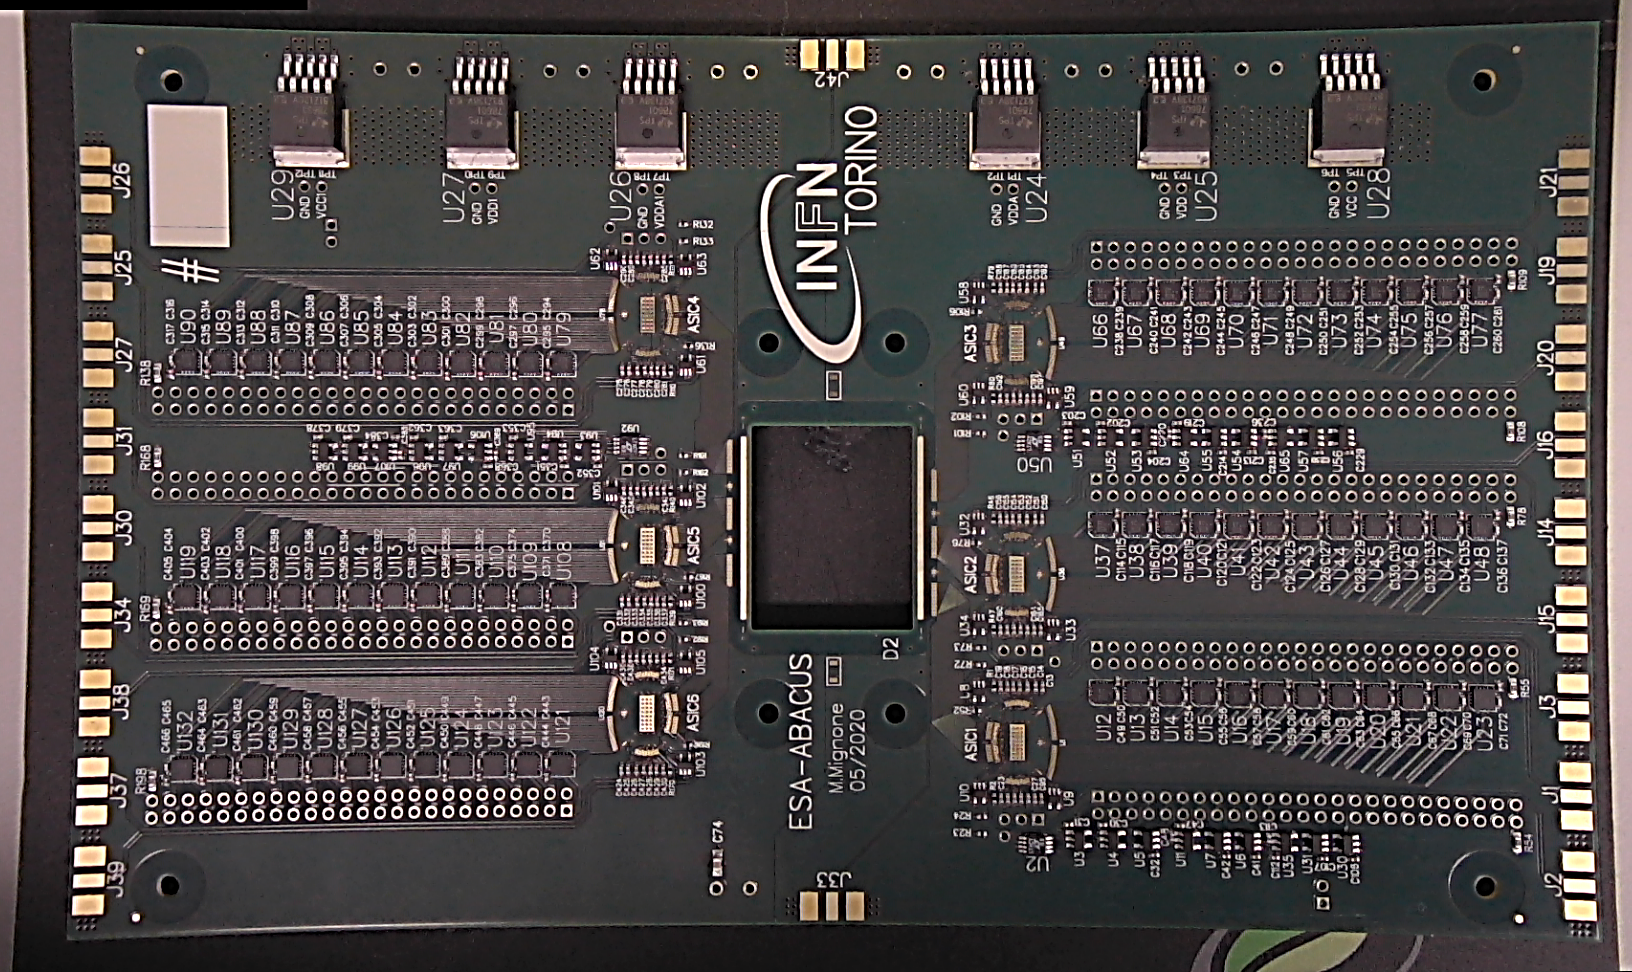
\includegraphics[width=0.7\linewidth]{IMG/ch2/EsaAbacus.png}
	\caption{Esa-Abacus board, chips and detector are not yet bonded.}
	\label{fig:esaabacus}
\end{figure}
\noindent Each FPGA board used has enough Input/Output resources for two ABACUS2 chips. This means that, in order to utilize at his full potential the ESA-ABACUS, three boards are needed.
The final goal is to use two of these devices placed in an orthogonal way in order to acquire the horizontal and vertical dispersion of the particle beam.
To be noted that this board, on the contrary of the ABACUS2 test board, is not intended for the validation of the chip, in fact it has no trimmers for any voltage regulation, instead it was made in order to test and utilize the 144 strip detector.
The output signals from the ABACUS2 chips use Current Mode Logic (CML) signalling standard, however the FPGA boards used for the readout only support Low Voltage Differential Signalling (LVDS) logic signals.
In order to make the chip and FPGA communicate each ESA-ABACUS board has CML-LVDS converters installed.


\section{FPGA board tasks}
\noindent As mentioned in previous sections, the digital data coming from the ABACUS2 chip are analysed by a Field Programmable Gate Array (FPGA) board, which is a programmable device that allows the end user to build complex electronic logic circuits without the need of specialized machinery.
For the MoVeIT project the FPGA firmware has three main tasks: 
\begin{itemize}
	\item it de-serialize the input data from the chip with a 1~GHz sampling rate (500~MHz clock in Double Data Rate (DDR)), it counts the transitions from \textit{low} to \textit{high} using a LookUp Table (LUT) and then it adds the result to a counter.
	This final value is the number of particles detected for a channel.
	The board does this process for each channel of the chip.
	In addition, by analysing the AND and OR logic combination serial data from two adjacent channels and using some maths it is possible to apply corrections to reduce the pile-up effects and to extend the measurable rate range; this will be very briefly explained in section \ref{structure};
	\item it configures the internal (trimming) DACs (see chapter 4) and the external DAC used to set the V$_{th}$.
	In addition, it controls the LCD display of the board, can read the board switches and buttons and it can turn on or off the board LEDs;
	\item it sends the data to a computer using User Datagram Protocol (UDP) via a Ethernet (RJ45) cable.  
\end{itemize}
















